\emph{Cancer} is an umbrella term for a group of diseases caused by abnormal cell growth in different parts of the body. The accumulation of extra cells usually forms a mass of tissue called a \emph{tumor}. Tumors can be benign or malignant: \emph{benign tumors} are noncancerous, lack the ability to invade surrounding tissue and will not regrow if removed from the body;  malignant or \emph{cancerous tumors} are harmful, can invade nearby organs and tissues (\emph{invasive cancer}), can spread to other parts of the body (\emph{metastasis}) and will sometimes regrow when removed~\cite{NCI2012}.

\emph{Breast cancer} forms in tissues of the breast. The two most common types of breast cancer are \emph{ductal carcinoma} and \emph{lobular carcinoma}, which start in the breast ducts and lobules, respectively (Fig.~\ref{fig:BreastAnatomy}). Breast cancer \emph{incidence rate}, the number of new cases in a specified population during a year, is the highest of any cancer among American women. Its \emph{mortality rate}, the number of deaths during a year, is also one of the highest of any cancer~\cite{Howlader2014}.

\begin{figure}[h]
	\centering
	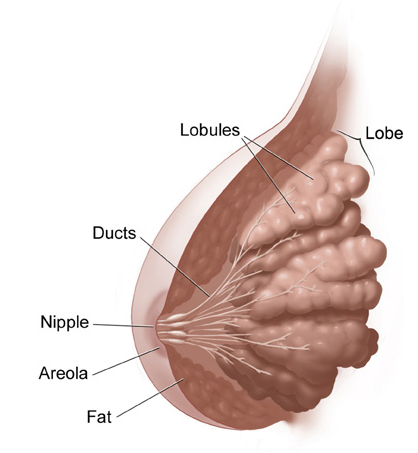
\includegraphics[width = 0.34\textwidth]{plots/breastAnatomy.png}
	\caption[Anatomy of the female breast]{Anatomy of the female breast. Image courtesy of~\cite{NCI2012}.}
	\label{fig:BreastAnatomy}
\end{figure}

The \emph{cancer stage} depends on the size of the tumor and whether the cancer cells have spread to neighboring tissue or other parts of the body. It is expressed as a Roman numeral ranging from 0 through IV; stage I cancer is considered \emph{early-stage breast cancer} and stage IV cancer is considered \emph{advanced}. Stage 0 describes non-invasive breast cancers, also known as \emph{carcinoma in situ}. Stage I, II and III describe invasive breast cancer, i.e., cancer has invaded normal, surrounding breast tissue. Stage IV is used to describe metastatic cancer, i.e., it has spread beyond nearby tissue to other organs of the body.

%\subsection{Mammograms}
\subsubsection{Mammograms}
A \emph{mammogram} is an x-ray image of the breast. Radiologists use \emph{screening mammograms} (normally composed of two mammograms of each breast) to check for breast cancer signs on women who lack symptoms of the disease. If an abnormality is found, a \emph{diagnostic mammogram} is ordered, these are detailed x-ray pictures of the suspicious region~\cite{NCI2014}. A standard mammogram is shown in Figure~\ref{fig:normalMammogram}.

\begin{figure}[h]
	\centering
	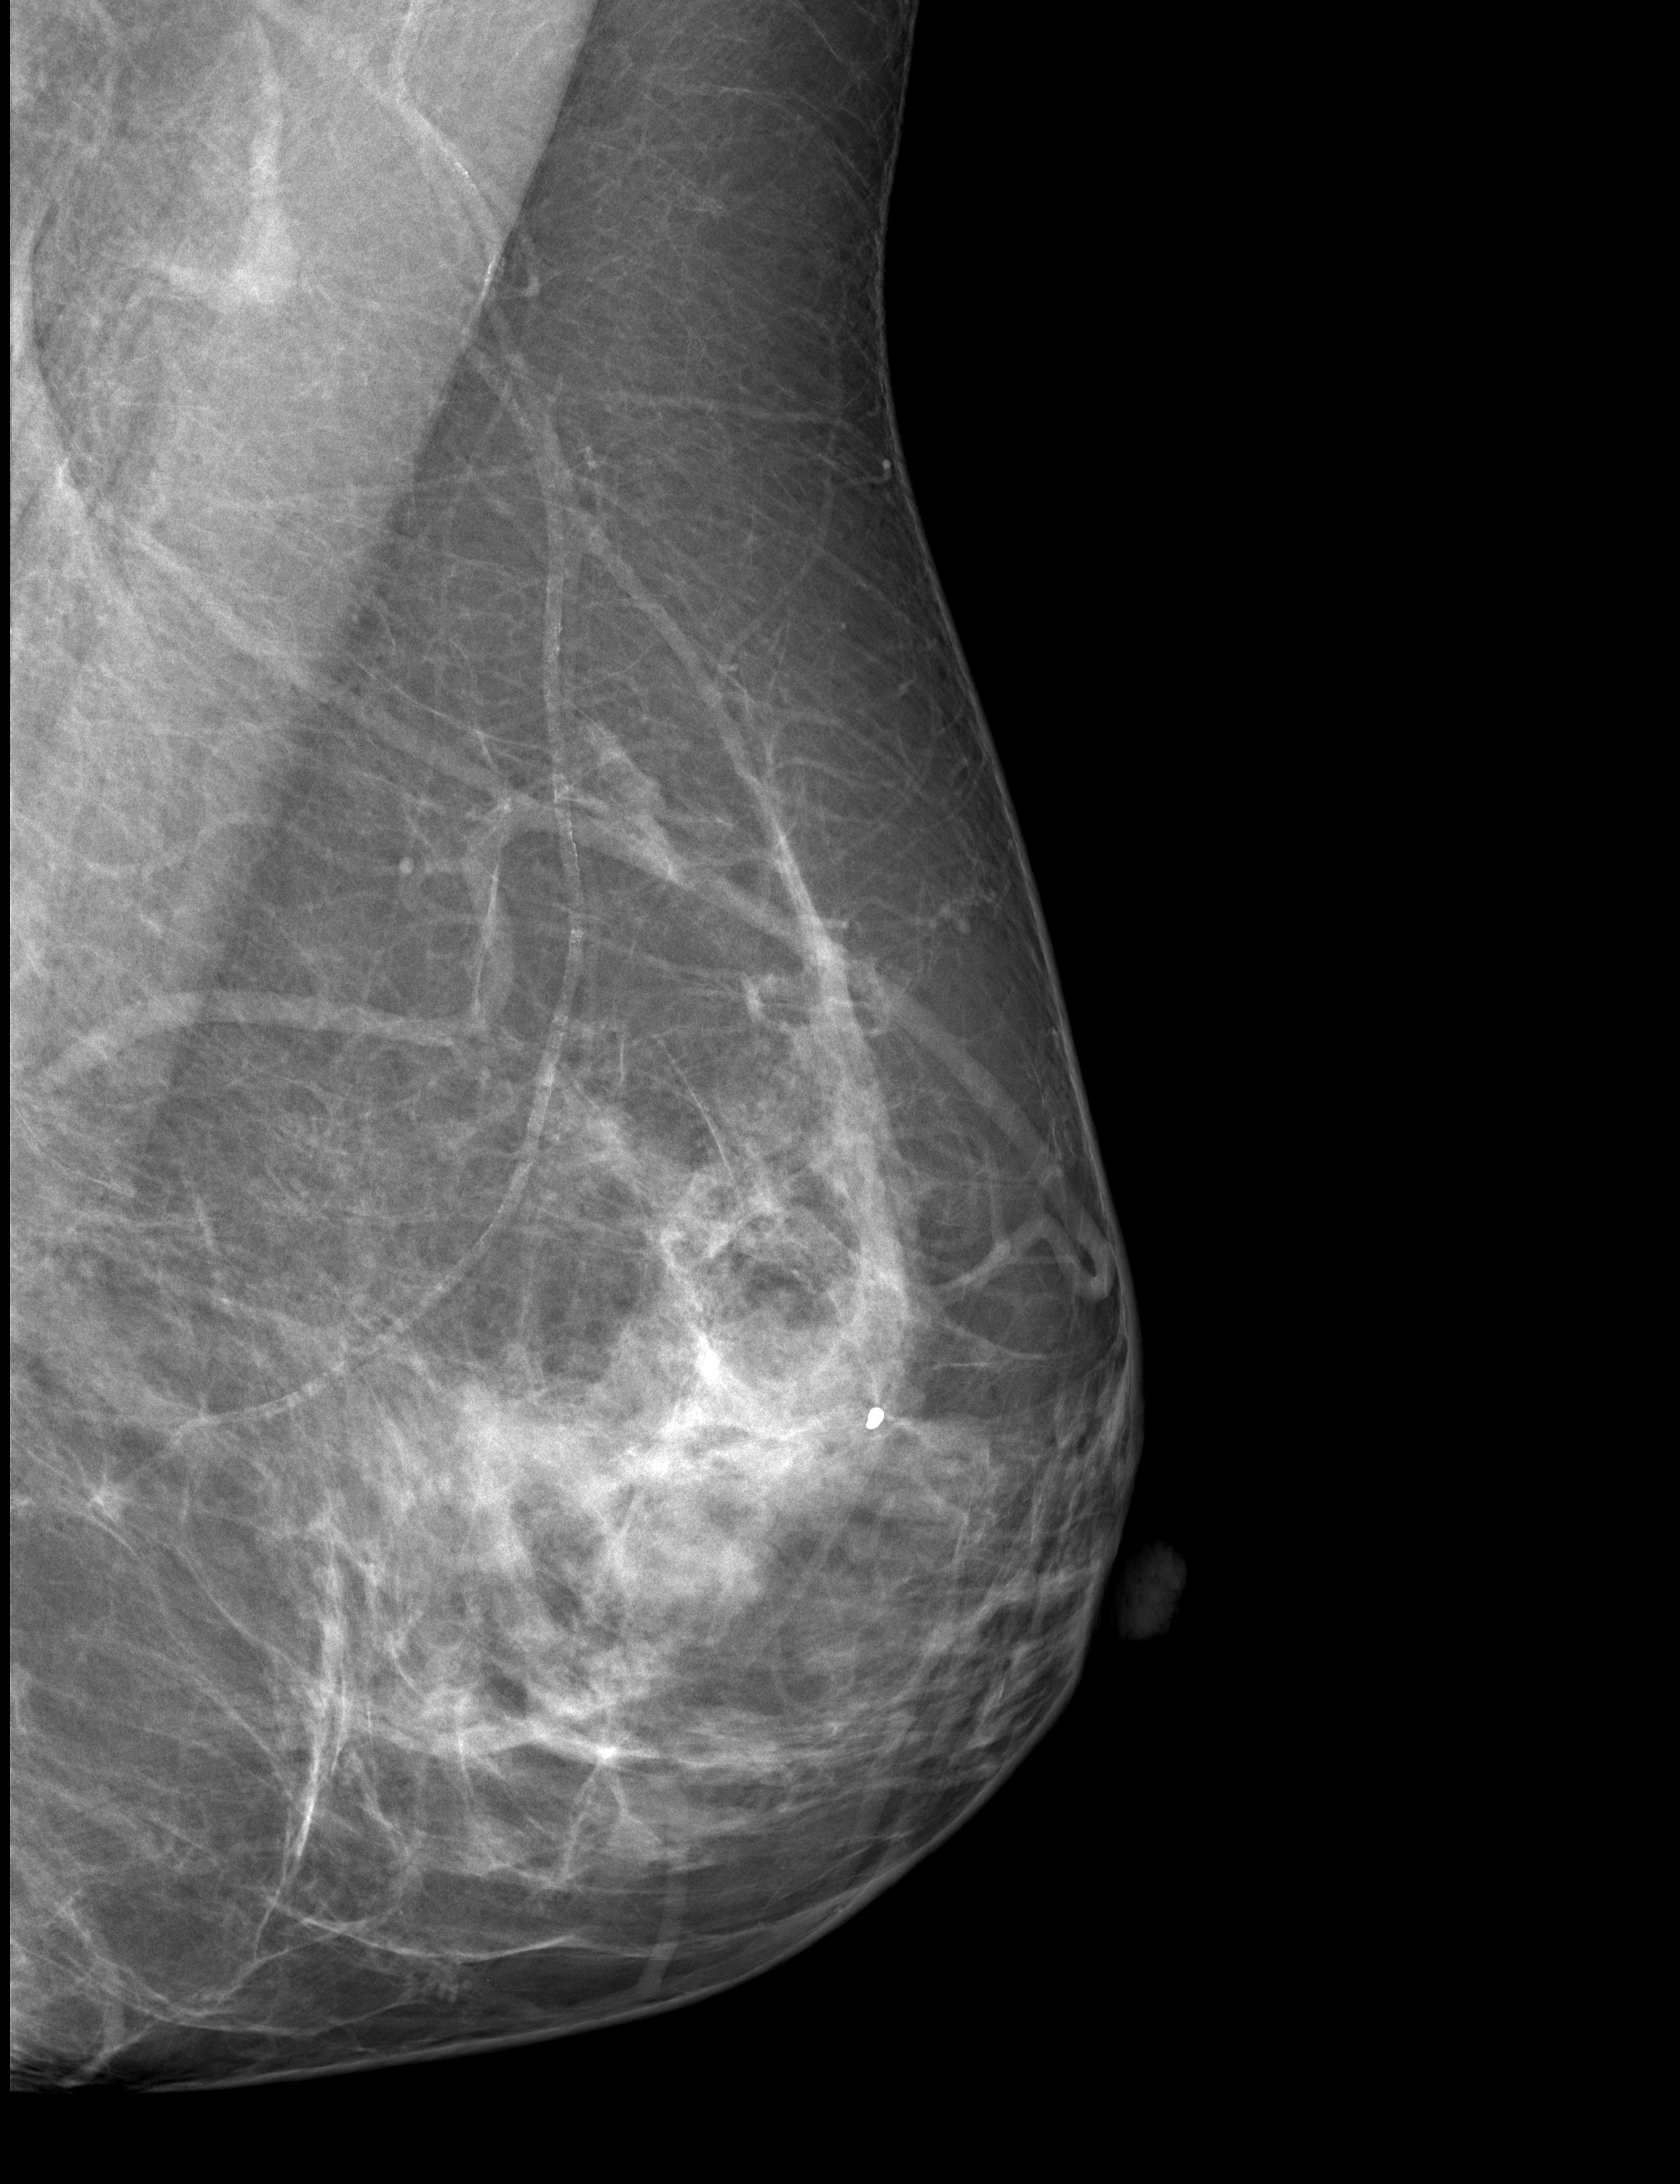
\includegraphics[width = 0.25\textwidth]{plots/normalMammogram.jpg}
	\caption[A digital mammogram]{A standard mammogram.}
	\label{fig:normalMammogram}
\end{figure}

Having a screening mammogram in a regular basis is the most effective method for detecting breast cancer early; around 85\% of breast cancers can be detected in a screening mammogram~\cite{BCSC2013}. Nevertheless, screening mammograms have many limitations: a high false positive rate, overtreatment in Stage 0 cancer, false negative results for women with high breast density, radiation exposure and physical and psychological discomfort~\cite{NCI2014}.

Radiologists look primarily for microcalcifications and breast masses. \emph{Microcalcifications} are tiny deposits of calcium in the breast tissue that can be a sign of early breast cancer if found in clusters with irregular layout and shapes (Fig.~\ref{fig:breastCancerSigns}). \emph{Breast masses} or breast lumps are a variety of things: fluid-filled cysts, fibric tissues, noncancerous or cancerous tumors, among others. A mass can be a sign of breast cancer if it has an irregular shape and poorly defined margins (Fig.~\ref{fig:breastCancerSigns}). Radiologists will also consider the breast density of the patient when reading a mammogram given that high breast density is linked to a higher risk of breast cancer~\cite{ACS2014}.
\begin{comment} My classification
Lesion
	Mass = Lump(This is palpable)
		Malignant = Cancerous
			Tumors
		Benign = Noncancerous
			Tumors
			Cysts
			Fibrosis/Fibroadenoma
	Microcalcifications (benign or malignant)

Tumors are abnormal growths of cells, cysts ae filled with fluid and fibrosis are "firmness in the connective tissues". Lesion is anything suspicious in a mammogram
Detection: Find lesions (malignant or benign)
Diagnosis: Find malignant lesions
\end{comment}

\begin{figure}[h]
	\centering
	\begin{subfigure}{0.24\textwidth}
                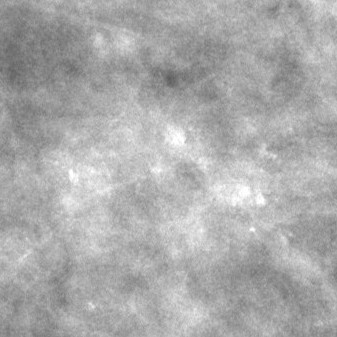
\includegraphics[width=\textwidth]{plots/breastMicrocalcification.jpg}
        \end{subfigure}
	~
	\begin{subfigure}{0.24\textwidth}
                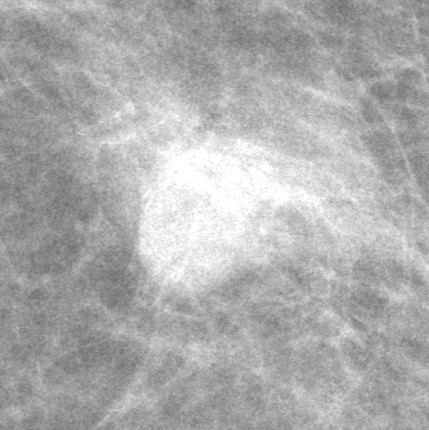
\includegraphics[width=\textwidth]{plots/breastMass.jpg}
        \end{subfigure}
	\caption[Signs of possible breast cancer]{Signs of possible breast cancer in a mammogram. Left: A cluster of microcalcifications in an irregular layout. Right: A poorly defined breast mass.}
	\label{fig:breastCancerSigns}
\end{figure}

Conventional mammography uses film to record x-ray images of the breast. \emph{Digital mammography}, on the other hand, uses digital receptors to convert the x-rays into electrical signals and stores the image electronically. Digital mammograms offer a clearer picture of the breast and can be digitally manipulated and shared between health care providers.
% However, researchers still debate whether [[its|their] use over| they] [surpass| improve on|outperform|[offers|have] an advantage over|are more effective than|benefit] film mammograms [in|for] [identifying breast cancer|breast cancer detection].
However, researchers still debate whether they offer an advantage over film mammograms~\cite{Kerlikowske2011, Pisano2008, Skaane2007}. Digital mammography is steadily becoming the standard for breast cancer screening. Figure~\ref{fig:normalMammogram} is, in fact, a digital mammogram.
\emph{Digital tomosynthesis}, also called three-dimensional mammography, is a new technology that produces 3-dimensional x-ray images of the breast and is expected to improve the efficacy of regular 2-d mammograms. Studies comparing the two techniques have not yet been published~\cite{NCI2014}.

\emph{Computer-aided detection} or \emph{CAD} systems inspect mammograms using computer algorithms: detection (CADe) looks for any lesion while diagnosis (CADx) focuses on malignant lesions.
They assist radiologists during mammography screening signaling suspicious areas and offering relevant information; however, whether accuracy improves is questioned~\cite{Lehman2015}.
% their value has been challenged

\begin{comment}
\subsection{Mammography databases}
\label{sec:BrCaDB}
Many public databases are available. We need them to train and evaluate our models.
% these are desired propertie, don't talkabotu we but about what is important or desired in a data abse.
Given the size of the expected network architecture and the data thirst of convolutional networks we focus only on the bigger databases. We also need pixel-level labels, i.e., lesions to be marked on each mammogram; this is generally made by expert radiologists drawing the boundaries of the lessions in the mammograms.
% Do I need to have perfect image segmentation?. Maybe not.
Furthermore, we prefer to have good contrast resolution, the number of gray colors represented per pixel, and good spatial resolution, the area represented per pixel: at least 12-bit images ($10^12 = 4048$ gray values per pixel) with 0.1-0.15 mm maximum pixel size. Greater constrast resolution means that more brightness values are captured per pixel while greater spatial resolution means that hopefully more detail is included in the image. Most mammography databases including all described below satisfy these conditions.

	The Digital Database for Screening Mammography (DDSM)~\cite{Heath2001} is arguably the most popular database used for CAD development. It is composed of around 10.5K digitised film mammograms from 2620 patients. Mammograms are either 12-bit or 16-bit images with 0.05 mm spatial resolution. Age and breast density of each patient is provided. Each lesion boundary is specified along with its information: type, assesment, subtlety and malignancy.
%Type is mass, microcalcification, assesment (1-5) in BIRADs, subtlety(1-5) and 

	The BancoWeb database~\cite{Nepomuceno2011} consists of around 1.5K digitised film mammograms from 300 patients although they claim other 5K images stored internally ``are being progressively transferred to the online database''~\footnote{This claim was made back in 2011 so we expect it to be done by now.}. Mammograms are 12-bit images with 0.075 or 0.15 mm pixel size. At the time of publishing (2011) only very few lesions had been marked in the mammograms and it was impossible to review the current state of the database given that its webpage was not accesible online, which could be a sign of permanent closure. The only advantage of this database and the reason we include it here is that it was collected in Brazil and may be useful to test our CAD in Latin American patients.

	The Breast Cancer Digital Repository (BCDR-DM) consists of 3.6K digital mammograms from 724 patients; this number was obtained from its website (\url{bcdr.eu/information/about}) which also states the database is still in construction and it is expected to have mammograms from 2000 to 3000 patients. Mammograms are 14-bit images with good spatial resolution~\footnote{The webpage does not explicitly states the image's spatial resolution but judging by the size of the entire images it is good enough.}. Each lesion outline is marked in the image along with its assesment and other relevant clinical data. They also have a fairly big repository of digitised film mammograms called BCDR-FM (3.7K) but at lower resolutions.
% Only has 270 patients(various studies), total 1K images, segmentations are found on image but no acces tfiles. Frick. Ask em for the other maybe.

	Another small digital mammogram repository is called INbreast~\cite{Moreira2012}. It consists of 410 digital mammograms from 115 patients. Each mammogram is a 14-bit image with 0.7 mm spatial resolution. Lesion boundaries are accurately marked and its information is also included. This could be used in conjunction with the BCDR-DM repository.

	Finally,~\cite{Zheng2012} used a private repository of around 6.5K digital mammograms obtained from 1120 patients. Specifics of contrast and spatial resolution are not provided but they are most probably good enough. Lesions are marked (with a circle) on the mammograms and lesion and patient information is provided. Even though this is a private repository of the University of Pittsburgh, if needed, we could ask them for access to it. This may not be plausible given the complications of sharing personal (granted anonymized) information and the size of the database.
%A small desciption is offered below.

% This should probably not go in
\paragraph{Alternatives}
We hope to obtain enough examples after cropping the mammograms into smaller image patches and applying some data augmentation to them (rotation and horizontal flipping). In case this is still not enough we could try various things: (1) obtain more labelled data from other sources, (2) reduce the complexity of the architecture to have less parameters to learn, (3) be more aggresive with the data augmentation, (4) pretrain the network with unlabelled digital mammograms which may be easier to get, (5) use film mammograms to pretrain the network and fine-tune it on digital mammograms and (6) use an already pretrained network in other similar domains and fine-tune it with digital mammograms.

Another option is to use only digitised film mammograms for the entire project but this will produce networks which expectedly produce bad results in digital mammograms~\cite{Zheng2012} and seems like a step in the wrong direction given the clear trend of hospitals replacing film mammography by digital mammography. A final option is to join film and digital mammograms into a single data set, this may or may not work given the difference between them but will most probably decrease the quality of results on digital mammograms when compared to a network trained only on digital mammograms.

\begin{comment}
Film Mammograms 
MIAS, DDSM, BancoWeb, CALMA, AMDI, B-screen, MiRAcle, BCDR-FM
inBeast paper has a good summary.

Digital 
INBreast, MIDAS (no labels), BCDR-DM

Clinical features: age, breast density, and family breast cancer history. 

Zheng2012 also says that "direct application of an SFM image-based CAD scheme to the FFDM images resulted in the substantial degradation of performance" "digitised image-based CAD can be converted for FFDMs while performing at a comparable, or better, level" "This is largely due to better contrast resolution, detection quantum efficiency and system linearity." He means converted as in retrained, though. (the ANN is completely retrained but it has little params)

Benchmarking datasets:
Moura, D.C., Loṕez, M.A.G., Cunha, P., De Posada, N.G., Pollan, R.R., Ramos, I., Loureiro, J.P., Moreira, I.C., De Araújo, B.M.F., Fernandes, T.C. Benchmarking datasets for breast cancer computer-aided diagnosis (CADx) (2013) Lecture Notes in Computer Science (including subseries Lecture Notes in Artificial Intelligence and Lecture Notes in Bioinformatics), 8258 LNCS (PART 1), pp. 326-333. 
show that 'this combination of clinical data and image descriptors is advantageous in most CADx scenarios.'
\end{comment}


% option: Adding mammography data bases as a subsection of breast cancer and upgrade mammograms as a subsection too. Make mammography databases small.
% option: do not add anything
\end{comment}

This section was written using information from the National Cancer Institute. We recommend to visit its website (\url{www.cancer.gov}) for further details.
